\subsection{Motion History}
\begin{table}[h!]
    \centering
    \begin{tabular}{ | l | c | c | c |}
        \hline
        Konfiguration & Beste Unter 50 kB & Unter 28 kB \\\hline
        Ensemble-Methode & ExtraTrees & & \\\hline
        Maximalhöhe & 10 & & \\\hline
        Waldgröße & 11 & & \\\hline
        ccp\_alpha & 0.0 & & \\\hline
        min\_samples\_leaf & 1 & & \\\hline
        Programmgröße in Bytes & -1 & & \\\hline
        Genauigkeit Testmenge von Klisch & 68.8\% & & \\\hline
        Genauigkeit Gestentestmenge & 71.5\% & & \\\hline
        Genauigkeit Nullgestentestmenge & 69.4\% & & \\\hline
    \end{tabular}
    \caption{Beste Konfigurationen der TODO.}
    \label{tab:TODO}
\end{table}
\begin{figure}[h!]
    \centering
    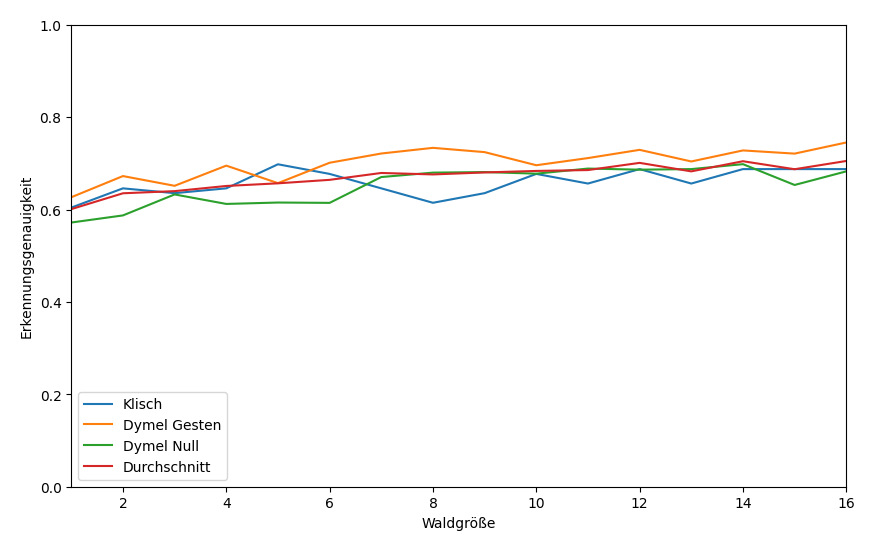
\includegraphics[width=\linewidth]{images/motion_history_acc_per_size.png}
    \caption{Die beste summierte Erkennungsgenauigkeit pro Waldgröße mit Motion History.}
    \label{fig:motion_history_per_forest_size}
\end{figure}
Die Featuremenge von Motion History beinhaltet für jeden Pixel einen Eintrag, die der Definition des Motion History Image folgen (siehe Formel \ref{formular:mhi}).
\newline
\newline
Zu erwarten war, dass Motion History am besten von allen Konfigurationen abschneidet, da es alle Anforderungen an ein Feature erfüllt. In der Praxis schneidet die Motion History allerdings am schlechtesten
im Hinblick auf die Erkennungsgenauigkeit der Testmenge von Klisch ab (siehe Tabelle \ref{tab:motion_history}). Die beste Ensemble-Methode ist ExtraTrees mit dieser Featuremenge. Allerdings ähnlich, wie die
Helligkeitsverteilung, ist der RandomForest insgesamt balancierter im Hinblick auf die Gestentestmenge von Dymel. Die Bagging Ensemble-Methode verursachte Fehler und konnte nicht evaluiert werden.
\newline
\newline
Motion History ist mit Gleitkommazahlen implementiert. Allerdings sollte es keine Probleme bereiten sie mit 8-Bit Integer zu reimplementieren. Damit sollte die Programmgröße deutlich sinken. Obwohl die
Konfiguration mit ExtraTrees am besten abschneidet, konnte die Konfiguration mit dem RandomForest nicht für den ATmega328P kompeliert werden aufgrund der Programmgröße. Es ist zu erwarten, dass dieser nach
der Reimplementierung klein genug ist.
\newline
\newline
In Abbildung \ref{fig:motion_history_per_forest_size} ist ein Anstieg der Erkennungsgenauigkeit mit zunehmender Waldgröße für die Testmenge von Klisch und die Nullgestentestmenge von Dymel zu erkennen. Auffällig ist
die Erkennungsgenauigkeit der Gestentestmenge von Dymel, die zunehmend abnimmt. Die Abbildung zeigt pro Waldgröße immer die beste Konfiguration im Hinblick auf die summierte Erkennungsgenauigkeit der
Testmenge von Klisch und der Nullgestentestmenge von Dymel an. Dementsprechend nimmt sie für die ExtraTrees Methode ab, nicht aber für RandomForest und Boosting.

